% Secciones 7 a 9: parser, AST, errores (tarea R2) - autor: Persona A.
\section{Diseño e implementación del parser}

\subsection{Arquitectura}
\begin{center}\small
\begin{tabular}{@{}>{\raggedright\arraybackslash}p{4.4cm} >{\raggedright\arraybackslash}p{10.2cm}@{}}
\toprule
\textbf{Módulo} & \textbf{Responsabilidad} \\
\midrule
\texttt{lexer.py} & Texto $\to$ lista de \texttt{Token} (tipo, lexema, posición, línea, columna) terminada en \texttt{\$}. Error léxico para símbolos desconocidos. \\
\texttt{gramatica.py} & Lista \texttt{PRODUCCIONES}; \texttt{calcular\_first}, \texttt{calcular\_follow}, \texttt{construir\_tabla}; detección de conflictos. \\
\texttt{parser\_rd.py} & Parser predictivo por \textbf{descenso recursivo}; construye el \textbf{AST}. \\
\texttt{parser\_ll1.py} & Parser \textbf{dirigido por la tabla LL(1)} con pila; construye el árbol de derivación y una traza. \\
\texttt{arbol.py} & Clases del AST, árbol genérico, texto jerárquico y exportación a Graphviz. \\
\texttt{errores.py} & \texttt{ErrorLexico} y \texttt{ErrorSintactico} (mensaje, posición, línea, columna, puntero \texttt{\^{}}). \\
\texttt{main.py} & Interfaz de línea de comandos (archivo, texto, modo interactivo, opciones de visualización). \\
\texttt{casos\_prueba.py}, \texttt{ejecutar\_pruebas.py}, \texttt{test\_parser.py} & Casos, ejecutor con ambos parsers y pruebas unitarias. \\
\bottomrule
\end{tabular}
\end{center}
Ningún módulo usa bibliotecas de generación de parsers: solo la biblioteca estándar de Python
(\texttt{re}, \texttt{dataclasses}, \texttt{argparse}, \dots).

\subsection{Analizador léxico}
Parte de la función \texttt{analizador\_lexico} entregada por el docente (expresiones regulares nombradas combinadas en un patrón único).
Se ampliaron: el token \texttt{COMA}; números decimales; el \textbf{registro de posición} (offset, línea y columna) de cada token,
necesario para ubicar los errores; el token de fin \texttt{\$}; y mensajes léxicos con sugerencia (``¿quiso escribir \texttt{==}?'').

\subsection{Parser por descenso recursivo}
Hay \textbf{un método por cada no terminal}, y cada método implementa sus producciones; los comentarios del código indican el
número de producción. Los no terminales auxiliares (\textit{programa'}, \textit{condicion'}, \textit{termino'}, \textit{acciones'},
\textit{parametros}) se implementan como ciclos \texttt{while}, que equivalen a la recursión por la derecha de la gramática
pero (i)~no desbordan la pila de Python con programas largos y (ii)~permiten construir el AST con asociatividad izquierda.
Cuando la alternativa elegida es $\varepsilon$, el parser verifica que el lookahead pertenezca a FOLLOW del no terminal, para
informar el error en el punto exacto en que aparece.

\begin{center}\small
\begin{tabular}{@{}>{\raggedright\arraybackslash}p{6cm} >{\raggedright\arraybackslash}p{9.3cm}@{}}
\toprule
\textbf{Producciones} & \textbf{Método (\texttt{ParserDescendente})} \\
\midrule
1--3 \;(\textit{programa}, \textit{programa'}) & \texttt{programa()} \\
4 \;(\textit{regla}) & \texttt{regla()} \\
5--7 \;(\textit{condicion}, \textit{condicion'}) & \texttt{condicion()} --- ciclo \texttt{while OR} \\
8--10 \;(\textit{termino}, \textit{termino'}) & \texttt{termino()} --- ciclo \texttt{while AND} + verificación FOLLOW \\
11--13 \;(\textit{factor}) & \texttt{factor()} \\
14 \;(\textit{comparacion}) & \texttt{comparacion()} \\
15--18 \;(\textit{valor}) & \texttt{valor()} \\
19--21 \;(\textit{acciones}, \textit{acciones'}) & \texttt{acciones()} --- ciclo \texttt{while COMA} \\
22--24 \;(\textit{accion}, \textit{parametros}) & \texttt{accion()} --- ciclo \texttt{while} lookahead $\in$ FIRST(valor) \\
\bottomrule
\end{tabular}
\end{center}

\lstinputlisting[firstline=105, lastline=151, firstnumber=105, caption={Extracto de parser\_rd.py: condicion, termino y factor (niveles de precedencia).}]{../parser_rd.py}

\subsection{Parser dirigido por tabla LL(1)}
El segundo analizador usa la \emph{misma} lista de producciones: la tabla se genera automáticamente desde \texttt{gramatica.py} y se
interpreta con una pila (inicializada con \texttt{\$ programa}). Si el tope es un terminal, debe coincidir con el token actual; si es un
no terminal, se consulta $M[X,a]$, se reemplaza $X$ por el lado derecho de la producción (en orden inverso) y se agregan los
nodos hijos al árbol de derivación. Una celda vacía produce un error que lista los terminales esperados (la fila de la tabla).
La opción \texttt{--traza} imprime cada paso (pila, entrada restante, acción); ver la captura del Anexo~B.

\lstinputlisting[firstline=47, lastline=87, firstnumber=47, caption={Extracto de parser\_ll1.py: bucle principal del analizador LL(1).}]{../parser_ll1.py}

\subsection{Coherencia entre gramática, informe y código}
La lista \texttt{PRODUCCIONES} es la \emph{única} fuente de verdad: de ella salen FIRST, FOLLOW, la tabla, el parser LL(1) y las tablas de este
informe (generadas por \texttt{informe/generar\_informe.py}). El parser por descenso recursivo se escribió a mano siguiendo cada
producción, y la suite de pruebas comprueba que ambos analizadores aceptan y rechazan exactamente las mismas entradas
(46 casos).

\section{Árbol sintáctico / AST}

El sistema construye dos representaciones:
\begin{itemize}[nosep]
\item \textbf{Árbol de derivación} (concreto), generado por el parser LL(1): contiene todos los no terminales, incluidos los auxiliares y las hojas $\varepsilon$.
\item \textbf{AST} (abstracto), generado por el parser de descenso recursivo: elimina los no terminales auxiliares, los paréntesis y las hojas $\varepsilon$; los
operadores son nodos internos y la asociatividad izquierda queda explícita (\texttt{Or(Or(a,b),c)}).
\end{itemize}
Ambos pueden mostrarse como texto jerárquico o exportarse a Graphviz (\texttt{--dot}).

\subsection{AST de la regla del enunciado}
Entrada: \texttt{WHEN temperatura > 28 AND humedad < 40 THEN encender ventilador;}
{\small
\begin{verbatim}
Programa
└── Regla (línea 1)
    ├── Condición
    │   └── AND
    │       ├── >
    │       │   ├── temperatura  [ID]
    │       │   └── 28  [NUM]
    │       └── <
    │           ├── humedad  [ID]
    │           └── 40  [NUM]
    └── Acciones
        └── Acción: encender
            └── objeto: ventilador
\end{verbatim}}
\begin{figure}[H]
\centering
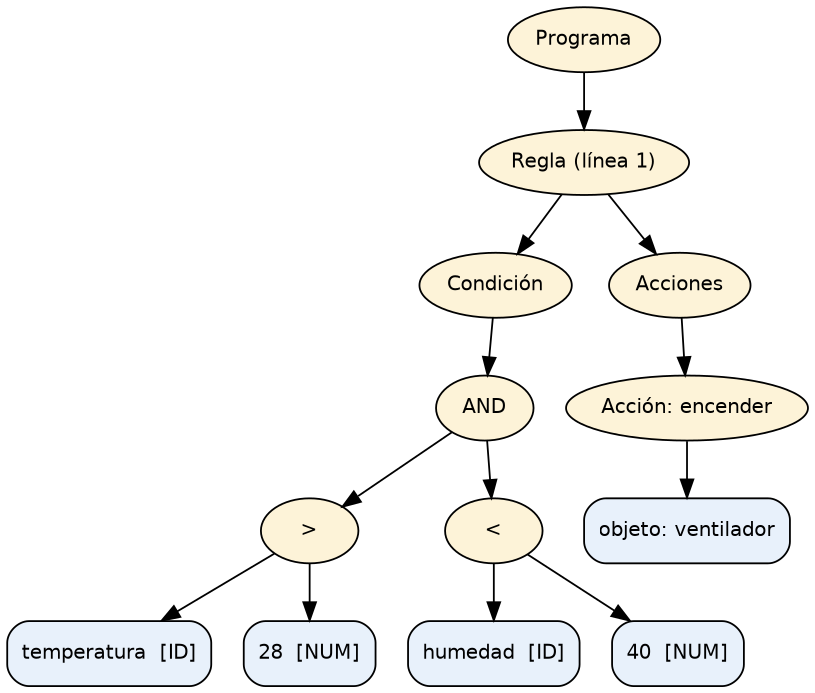
\includegraphics[width=0.55\textwidth]{../docs/img/ast_enunciado.png}
\caption{AST generado (Graphviz) para la regla del enunciado. Óvalos: nodos internos; cajas: hojas.}
\end{figure}

\subsection{AST con la extensión (NOT, paréntesis, acciones múltiples con parámetros)}
Entrada: \texttt{WHEN NOT (puerta == TRUE) AND (hora >= 22 OR hora < 6) THEN bloquear puerta\_principal, ajustar termostato 22;}

Se observa que el AST refleja la precedencia (\texttt{AND} es la raíz de la condición; \texttt{OR} queda dentro del segundo operando por los paréntesis)
y que los paréntesis no aparecen como nodos: su efecto está en la forma del árbol.
\begin{figure}[H]
\centering
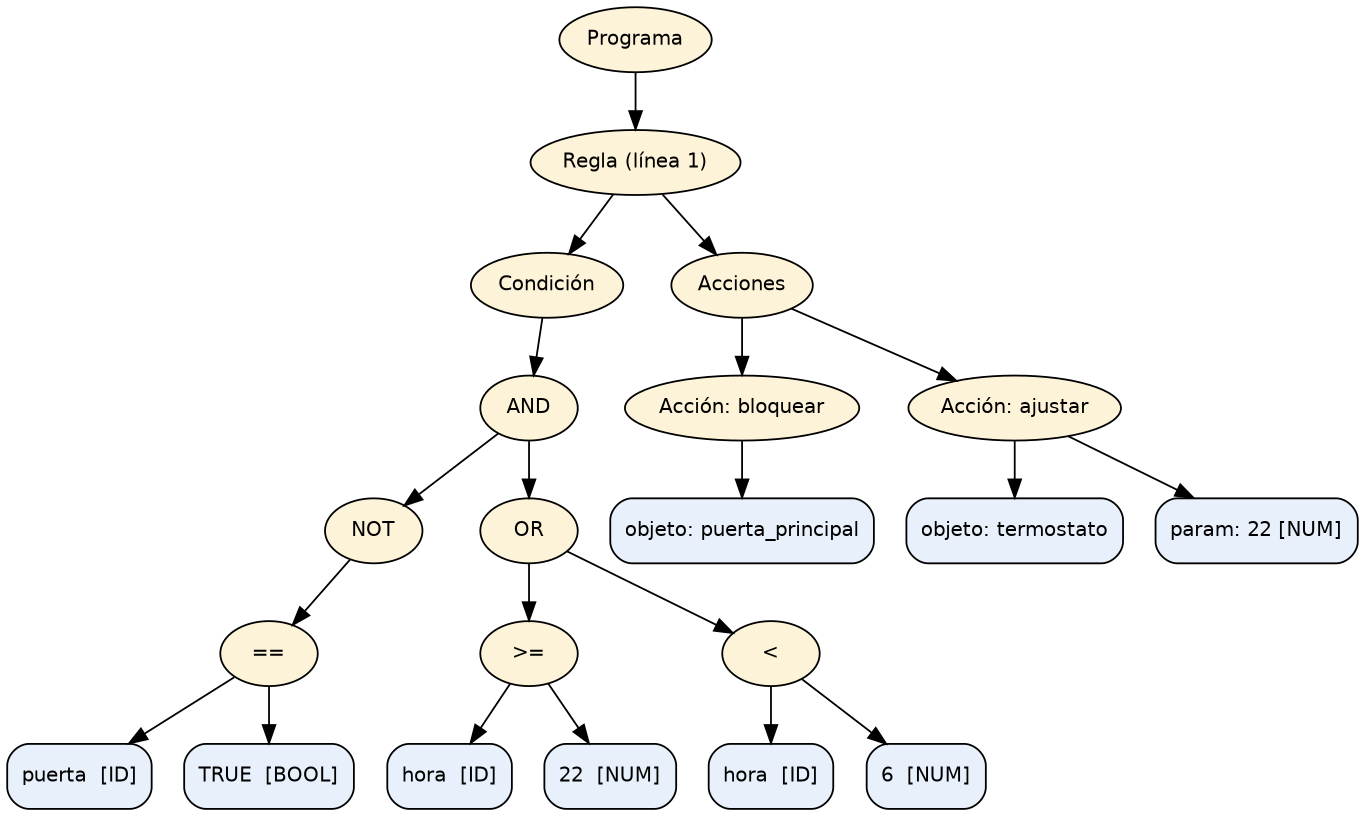
\includegraphics[width=\textwidth]{../docs/img/ast_extension.png}
\caption{AST de una regla con \texttt{NOT}, paréntesis, dos acciones y un parámetro.}
\end{figure}

\subsection{Árbol de derivación (parser LL(1))}
Para \texttt{WHEN a > 1 THEN x y;}; las hojas $\varepsilon$ corresponden a las producciones vacías 3, 7, 10, 21 y 24.
\begin{figure}[H]
\centering
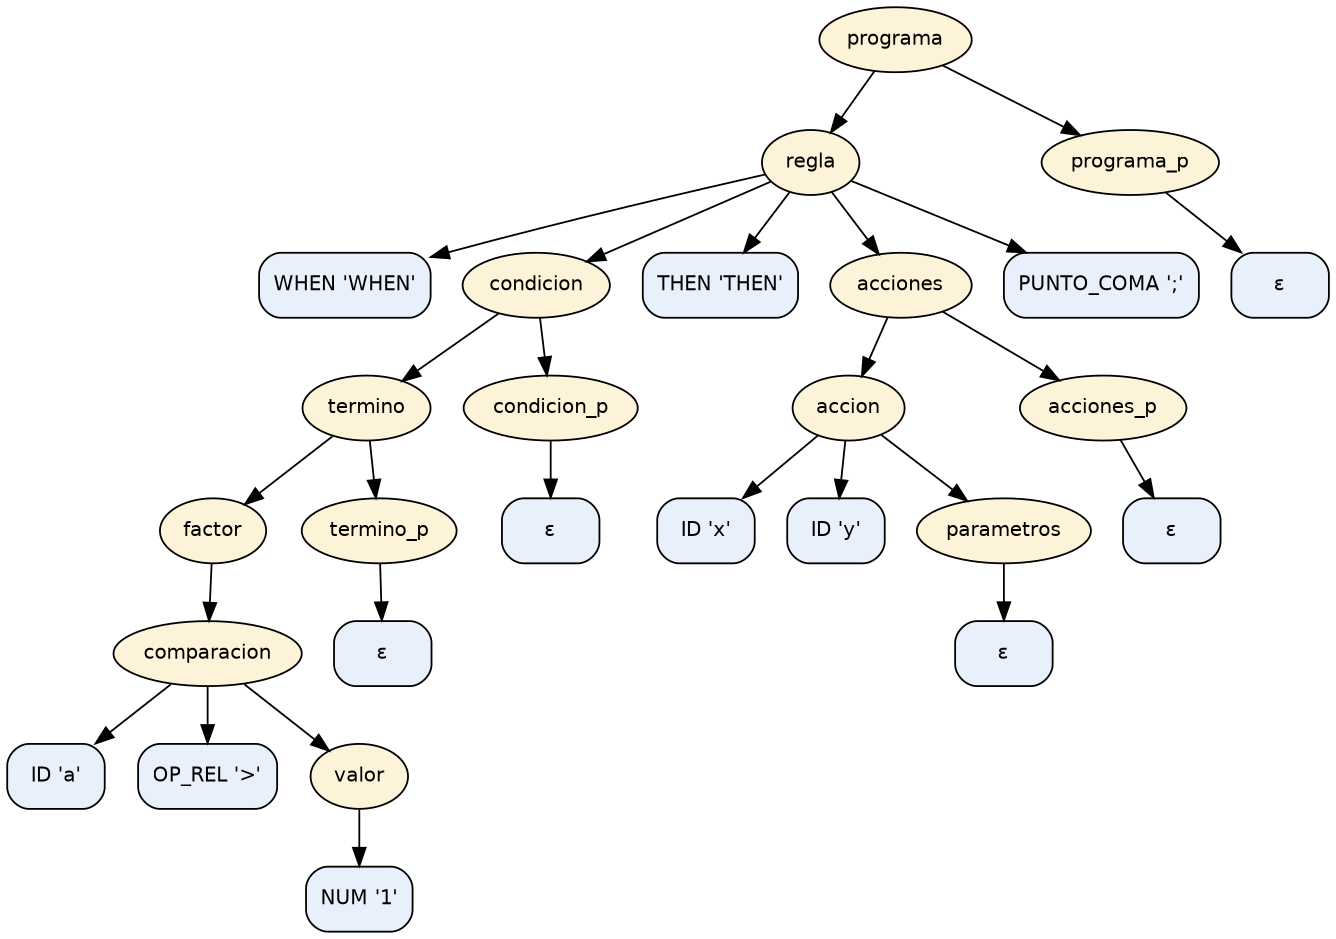
\includegraphics[width=\textwidth]{../docs/img/derivacion_simple.png}
\caption{Árbol de derivación obtenido con la tabla LL(1).}
\end{figure}

\section{Manejo de errores}

\paragraph{Estrategia.} El analizador se detiene en el \textbf{primer error} y lo informa con tres datos de ubicación
(línea, columna y posición/offset), el mensaje, la línea de código afectada y un puntero \texttt{\^{}} bajo el token problemático.
Hay dos clases de error: \texttt{ErrorLexico} (carácter fuera del alfabeto) y \texttt{ErrorSintactico}.
Los mensajes siguen el formato \emph{se esperaba} $X$ \emph{[contexto]}, \emph{pero se encontró} $Y$, y dependen del contexto sintáctico:
\begin{itemize}[nosep]
\item Después de la condición se pide \texttt{THEN} (o un conector AND/OR) y, dentro de un paréntesis, se pide \texttt{)} indicando la columna donde se abrió.
\item Un \texttt{)} sin \texttt{(} se informa como ``paréntesis de cierre sin su \texttt{(} correspondiente''.
\item Cada punto de la gramática tiene su mensaje: valor tras el operador, operador tras el identificador, dispositivo tras la acción, \texttt{;} al final, etc.
\item La entrada vacía tiene un mensaje propio.
\end{itemize}
La notación $[l{:}c]$ indica línea y columna. En el programa, el mensaje completo incluye también la posición (offset).

\subsection{Mensajes del analizador de descenso recursivo}
\begin{longtable}{@{}l >{\raggedright\arraybackslash}p{5.2cm} >{\raggedright\arraybackslash}p{8.4cm}@{}}
\toprule
\textbf{Caso} & \textbf{Entrada} & \textbf{Mensaje entregado por el analizador} \\
\midrule
\endhead
I01 & \footnotesize \texttt{WHEN temperatura > 28 encender ventilador;} & \footnotesize Error sintáctico [1:23]: se esperaba la palabra reservada THEN (o un conector AND / OR) después de la condición, pero se encontró el identificador 'encender'. \\
\addlinespace[2pt]
I02 & \footnotesize \texttt{WHEN temperatura > THEN encender ventilador;} & \footnotesize Error sintáctico [1:20]: se esperaba un valor (número, TRUE, FALSE o identificador) después del operador >, pero se encontró la palabra reservada THEN. \\
\addlinespace[2pt]
I03 & \footnotesize \texttt{WHEN temperatura 28 THEN encender ventilador;} & \footnotesize Error sintáctico [1:18]: se esperaba un operador relacional ('>', '<', '>=', '<=', '==', '!=') después de 'temperatura', pero se encontró el número 28. \\
\addlinespace[2pt]
I05 & \footnotesize \texttt{WHEN temperatura > 28 THEN encender ventilador} & \footnotesize Error sintáctico [1:47]: se esperaba ';' al final de la regla (o ',' para encadenar otra acción), pero se encontró el fin de la entrada. \\
\addlinespace[2pt]
I06 & \footnotesize \texttt{WHEN temperatura > 28 THEN ;} & \footnotesize Error sintáctico [1:28]: se esperaba el nombre de una acción (identificador) después de THEN, pero se encontró el símbolo ';'. \\
\addlinespace[2pt]
I07 & \footnotesize \texttt{WHEN temperatura > 28 THEN encender;} & \footnotesize Error sintáctico [1:36]: se esperaba el dispositivo u objeto (identificador) después de la acción 'encender', pero se encontró el símbolo ';'. \\
\addlinespace[2pt]
I08 & \footnotesize \texttt{WHEN (temperatura > 28 THEN encender ventilador;} & \footnotesize Error sintáctico [1:24]: se esperaba ')' para cerrar el paréntesis abierto en la columna 6, pero se encontró la palabra reservada THEN. \\
\addlinespace[2pt]
I09 & \footnotesize \texttt{WHEN temperatura > 28) THEN encender ventilador;} & \footnotesize Error sintáctico [1:22]: paréntesis de cierre ')' sin su '(' correspondiente. \\
\addlinespace[2pt]
I10 & \footnotesize \texttt{WHEN temperatura > 28 AND THEN encender ventilador;} & \footnotesize Error sintáctico [1:27]: se esperaba una condición (un identificador, NOT o '(') después de AND, pero se encontró la palabra reservada THEN. \\
\addlinespace[2pt]
I15 & \footnotesize \texttt{WHEN temperatura > 28 THEN encender ventilador @;} & \footnotesize Error léxico [1:48]: símbolo no reconocido '@'. \\
\addlinespace[2pt]
\bottomrule
\end{longtable}

\subsection{Mensajes del analizador dirigido por tabla}
El parser LL(1) usa un mensaje más genérico, construido a partir de la fila de la tabla (los terminales para los que existe producción):

\begin{longtable}{@{}l >{\raggedright\arraybackslash}p{4.4cm} >{\raggedright\arraybackslash}p{9.2cm}@{}}
\toprule
\textbf{Caso} & \textbf{Entrada} & \textbf{Mensaje del analizador dirigido por tabla} \\
\midrule
\endhead
I01 & \footnotesize \texttt{WHEN temperatura > 28 encender ventilador;} & \footnotesize Error sintáctico [1:23]: símbolo inesperado: se encontró el identificador 'encender'; en este punto (<termino\_p>) se esperaba la palabra reservada THEN, AND, OR o ')'. \\
\addlinespace[2pt]
I02 & \footnotesize \texttt{WHEN temperatura > THEN encender ventilador;} & \footnotesize Error sintáctico [1:20]: símbolo inesperado: se encontró la palabra reservada THEN; en este punto (<valor>) se esperaba TRUE, FALSE, un identificador o un número. \\
\addlinespace[2pt]
I10 & \footnotesize \texttt{WHEN temperatura > 28 AND THEN encender ventilador;} & \footnotesize Error sintáctico [1:27]: símbolo inesperado: se encontró la palabra reservada THEN; en este punto (<factor>) se esperaba NOT, un identificador o '('. \\
\addlinespace[2pt]
\bottomrule
\end{longtable}

Ambos analizadores coinciden siempre en \emph{aceptar o rechazar}; el de descenso recursivo da mensajes más específicos porque conoce el contexto
(el motivo por el que se llegó a cada método). Las capturas de los Anexos~B muestran el formato real, con puntero.

\paragraph{Limitación.} No hay recuperación de errores (modo pánico): tras el primer error el análisis termina. Sería una extensión natural
sincronizar en \texttt{;} (que pertenece a FOLLOW de \textit{acciones}) para informar varios errores por ejecución.

